

\documentclass[oneside,a4paper,12pt]{article}

\usepackage[]{hyperref}
\usepackage{tikz}
\usetikzlibrary{arrows,shapes,snakes,automata,backgrounds,petri}
\usepackage[utf8]{inputenc}
\usepackage{tabularx}
\usepackage{textcomp}
\usepackage{amsmath}
\usepackage{float}
\newcolumntype{M}[1]{>{\centering\arraybackslash}m{#1}}

\usepackage[nottoc,notlot,notlof,numbib]{tocbibind}
\usepackage[titletoc]{appendix}
\usepackage{titletoc}
\renewcommand{\appendixname}{Annexure}
\renewcommand{\bibname}{References}
\setcounter{secnumdepth}{5}

\usepackage{float}
\usepackage{subcaption}
\usepackage{multirow}

\usepackage[ruled,vlined]{algorithm2e}

\begin{document}

\setlength{\parindent}{0mm}
\begin{center}

\includegraphics[width=100pt]{IIT_Bombay_color_logo.png} \\
\vspace{20pt}
{\bfseries INDIAN INSTITUTE OF TECHNOLOGY BOMBAY \\}
 \vspace*{2\baselineskip}
{\bfseries Project Report on \\}
 \vspace*{1\baselineskip}
{\bfseries \fontsize{16}{12} \selectfont  INSTI-BLOG \\ \vspace*{2\baselineskip}}
{\fontsize{12}{12} \selectfont SUBMITTED TOWARDS THE
 \\PARTIAL FULFILLMENT OF THE REQUIREMENTS OF \\

\vspace*{2\baselineskip}}
{\bfseries \fontsize{14}{12} \selectfont CS699:Software Lab (Computer Science and
Engineering) \\
\vspace*{1\baselineskip}} 
{\bfseries \fontsize{14}{12} \selectfont BY \\ 
\vspace*{1\baselineskip}} 

\begin{tabular}{l l}
\bfseries{Anurag Chaudhary}     &  \hspace{10mm}\bfseries{Roll No:193050061}\\
\bfseries{Himanshu Aswal}     &  \hspace{10mm}\bfseries{Roll No:193059001}\\
\bfseries{Sanyam Raj}     &  \hspace{10mm}\bfseries{Roll No:193050096}\\



\end{tabular}

\vspace*{2\baselineskip}
\vspace{20pt}

{\bfseries \fontsize{14}{12} \selectfont DEPARTMENT OF COMPUTER SCIENCE AND ENGINEERING \\
\vspace{20pt}}

\end{center}

\newpage



\begin{figure}[ht]
\centering

\includegraphics[width=100pt]{IIT_Bombay_color_logo.png}
\end{figure}


{\bfseries \fontsize{14}{12} \selectfont \centerline{INDIAN INSTITUTE OF TECHNOLOGY BOMBAY}
\vspace{10pt}
\centerline{Department of Computer Science and Engineering}
\vspace*{2\baselineskip}} 


{\bfseries \fontsize{16}{12} \selectfont \centerline{CERTIFICATE} 
\vspace*{2\baselineskip}} 

\centerline{This is to certify that the Project Entitled}
\vspace*{.5\baselineskip} 

\begin{center}
{\bfseries \fontsize{14}{12} \selectfont {INSTI-BLOG}
\vspace*{1\baselineskip}
\\Submitted by
\vspace*{0.5\baselineskip}}

\begin{tabular}{l l}
\bfseries{Anurag Chaudhary}     &  \hspace{10mm}\bfseries{Roll No:193050061}\\
\bfseries{Himanshu Aswal}     &  \hspace{10mm}\bfseries{Roll No:193059001}\\
\bfseries{Sanyam Raj}     &  \hspace{10mm}\bfseries{Roll No:193050096}\\



\end{tabular}
\end{center}




is a bonafide work carried out by students and it
is submitted towards the partial fulfillment of the requirement of CS699:Software Lab (Computer Science and Engineering).\\

\bgroup
\def\arraystretch{0.7}
\vspace{35pt}


\begin{center}
%\fontsize{12}{18}\selectfont 
{
Prof. Kavi Arya
\\Department of Computer Science, IIT Bombay
}
\end{center}

\newpage
\tableofcontents
\newpage
\newpage
{  \newpage {\bfseries \fontsize{14}{12} \selectfont \centerline{Introduction} 
\vspace*{2\baselineskip}} \setlength{\parindent}{11mm} }
{ \setlength{\parindent}{0mm} }
Our Institute has bunches of imaginative personalities and every one has a varied and an intriguing interpretation of a point or subject and these perspectives must reach out to everybody on the campus and each one must know about the happenings in the surroundings. 
\\\\There is no basic application where students can pursue the posts of different understudies regular to their advantage. This application will offer updates to the understudies as and when somebody presents any blog related on the interests specified by the student. 
\\\\Any happenings or posts related on any enthusiasm of the student is posted on whatsapp which is exceptionally vague now and then to pursue and can stir up alongside the messages and individuals can miss significant updates. This gives a platform on which there are just posts and nothing else so it will be anything but difficult to pursue the updates and blogs. 
\\\\The blogs and events identified with the enthusiasm of an student can be informed and the enrollment of the events should be possible on the same platform instead of forms being floated on whatsapp and mails. Students can catch up even after missing on the posts or events posted by somebody.
\\\\To facilitate all these, we have come up with an idea of a web application which gives a platform to the students to express their perspectives regarding a matter of their interest and furthermore follow subjects of their interest to realize the happenings specific to their point of interest, all at one place. The application gives space to compose writes on any theme of decision and others can pursue and can even express their perspectives on a specific blog by somebody.




%\justifying
\noindent
\vfill
\setlength{\parindent}{11mm}
\newpage
\section{Problem Statement}
\begin{itemize}
    \item In the institute, sometimes gatherings and discussions for various clubs takes place and most often the interested student may miss out on those due to their commitments to academic/personal stuffs.
    \item The announcement for events are sometimes on webmail/gmail or even whatsapp which may get mixed along with the messages and student may miss important updates for the event.
    \item An interested newbie may sometimes not put his points in the club gatherings.

\end{itemize}



\section{Motivation}
\begin{itemize}
    \item Summary of gathering and discussion should somehow reach each and everyone interested on campus.
\item Updates about each and every event of a specific interest, all at one place is convenient.
\item A medium or a platform to voice views and concerns and exhibit creativity on any subject of interest.

\end{itemize}

\section{User Documentation}
The source code can be downloaded directly from the github link: \url{https://github.com/anurag199831/Blog_app}.
The required modules are specified in the requirements.txt file and the commands to download the required modules are mentioned in readme file.
\\\\The user has to login using his/her google ID and then select the categories of interest. The user is then directed to the homepage where all the posts sorted in order of the date and time of posting are displayed. The users can post blogs with multiple tags. The users can also post images and videos as blog posts.

\newpage  
\begin{figure}[h]
\centering
    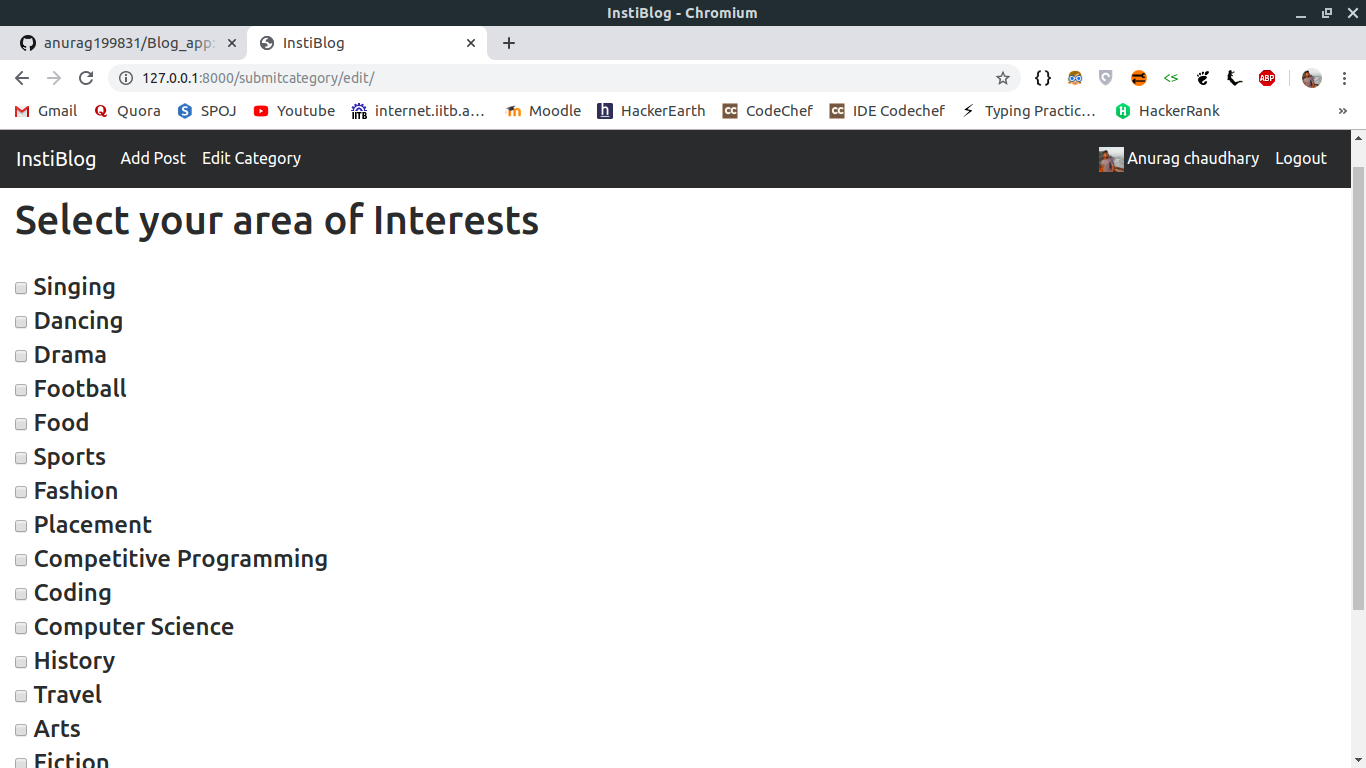
\includegraphics[scale=0.2]{SS1.png}
    \caption{Selecting categories after SignUp}
   \vspace{1em}
    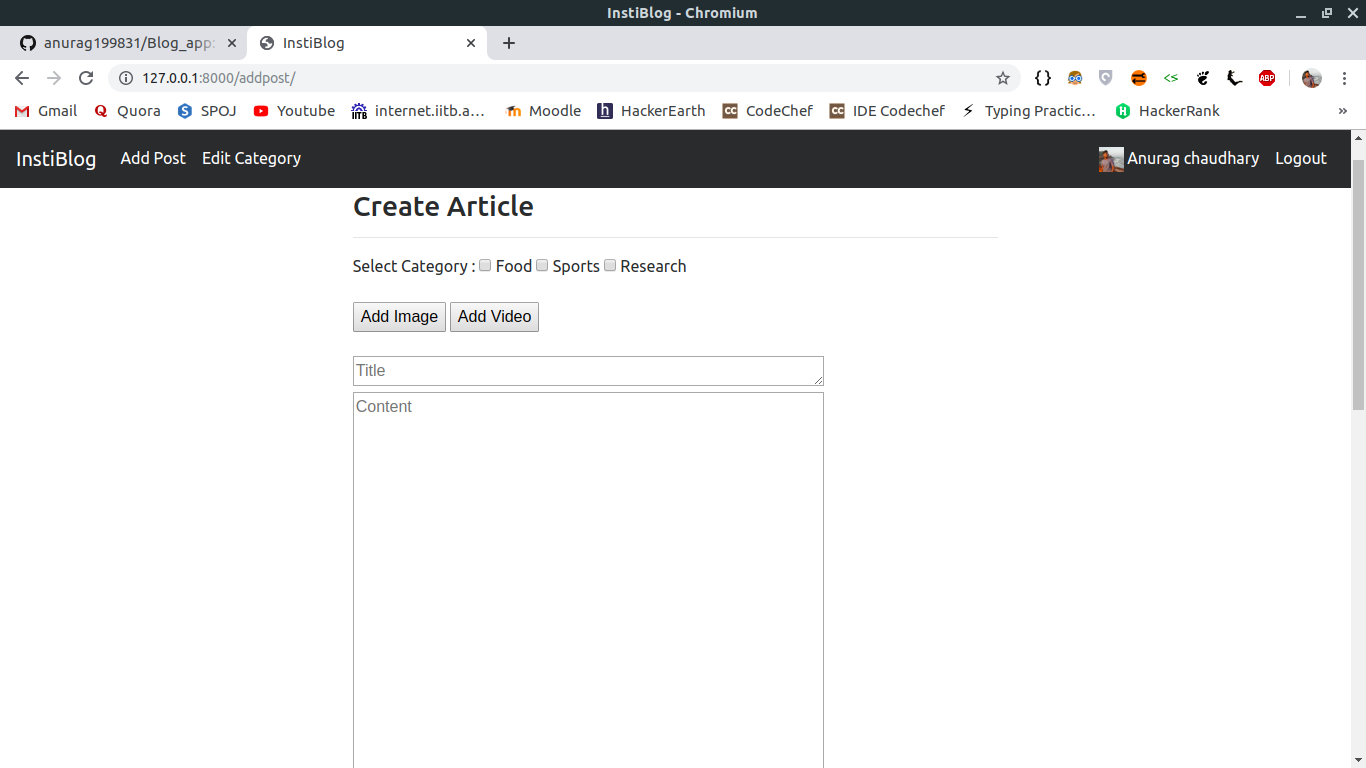
\includegraphics[scale=0.2]{SS2.png}
    \caption{Creating a new Blog Post}
\end{figure}

\newpage
\begin{figure}[H]
\centering
    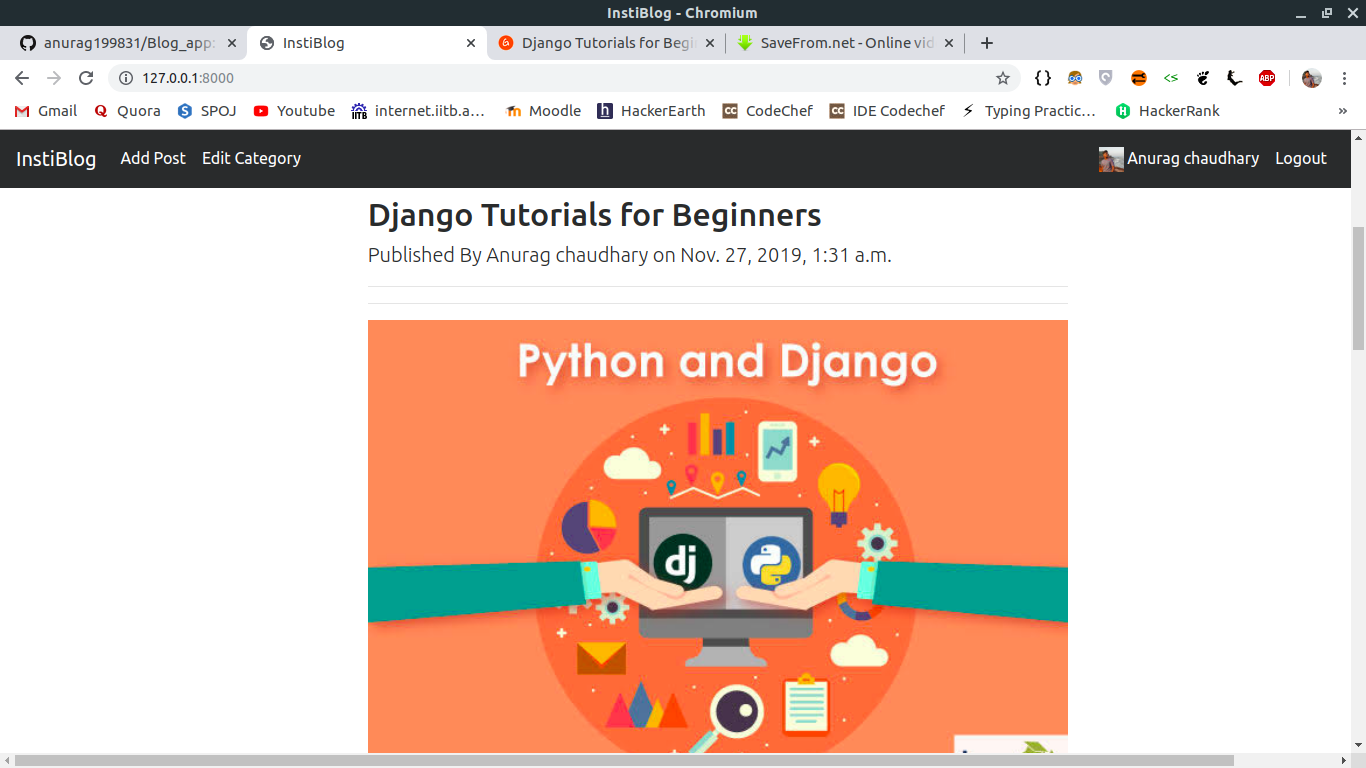
\includegraphics[scale=0.2]{SS3.png}
    \caption{Image in a Blog }
    \vspace{1em}
    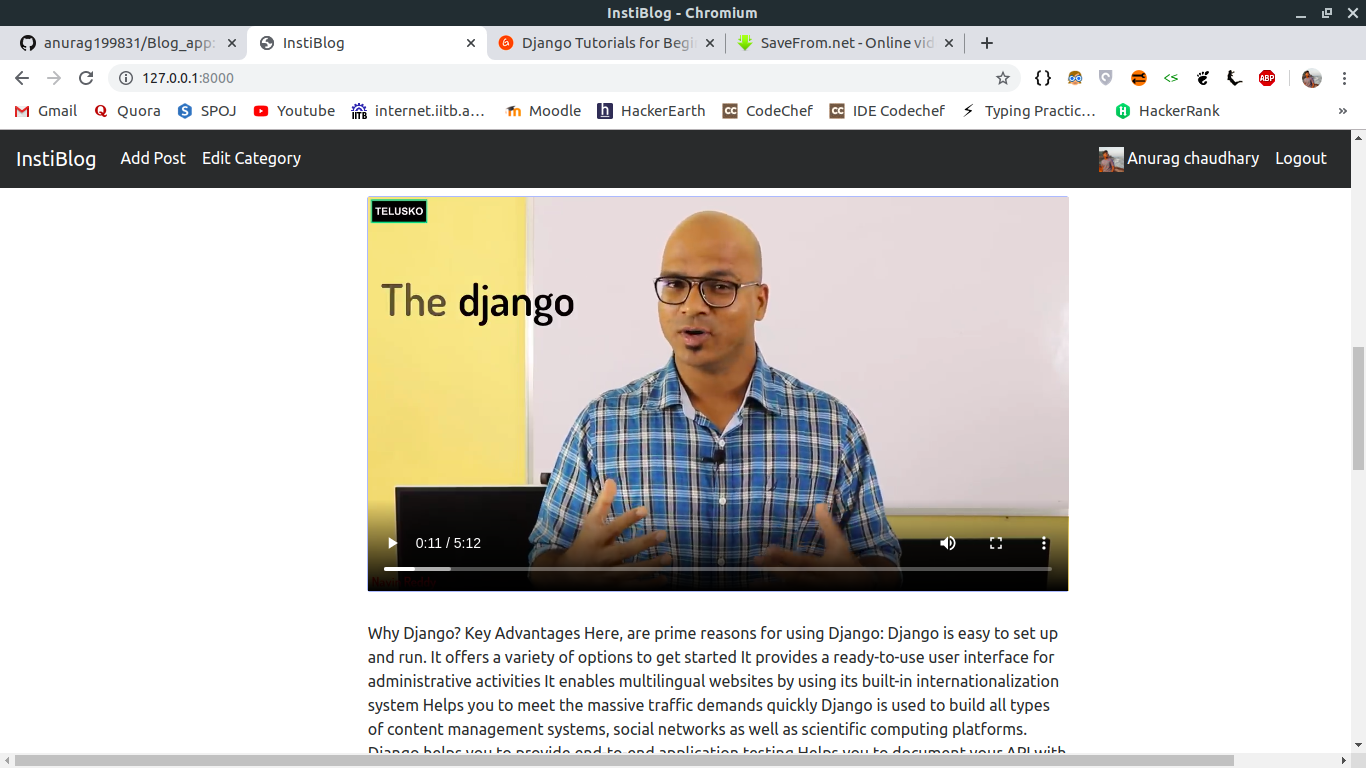
\includegraphics[scale=0.2]{SS4.png}
    \caption{Video in a Blog}
    \vspace{1em}
    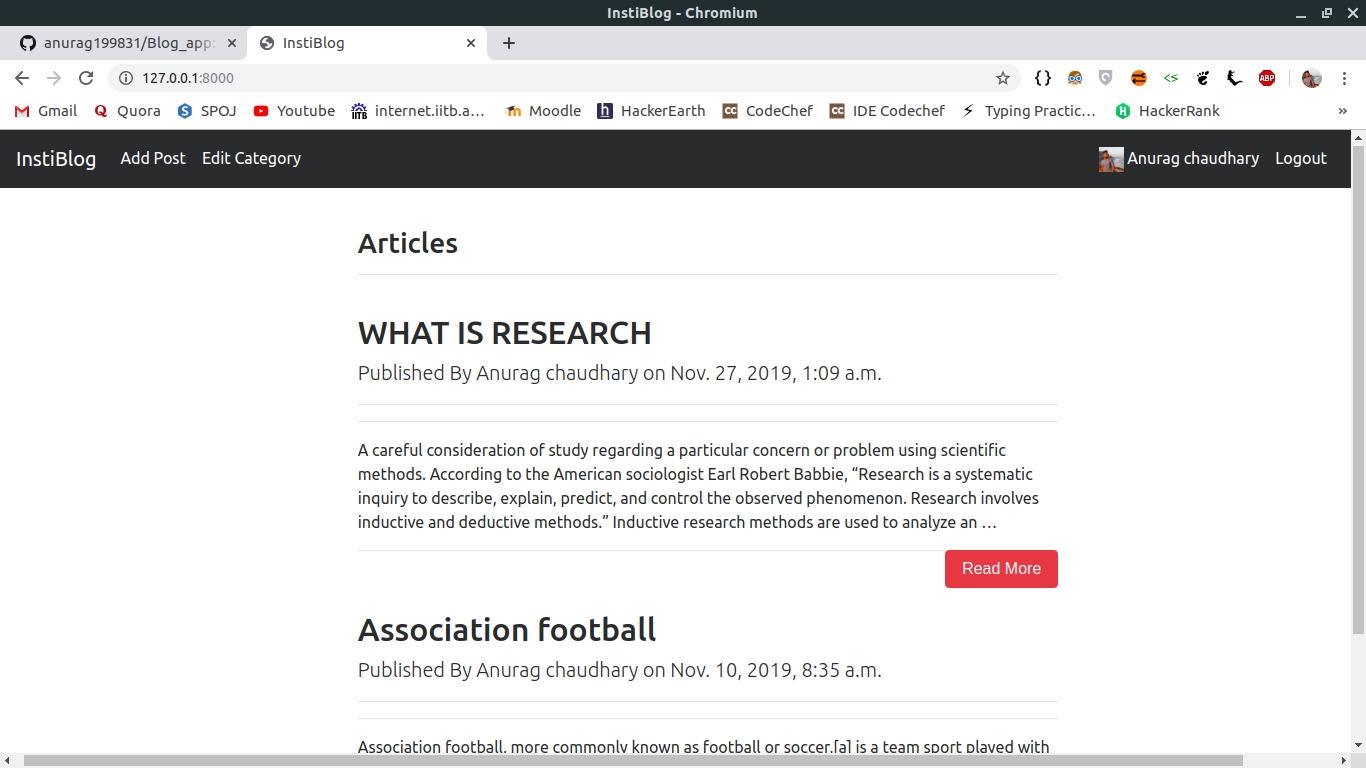
\includegraphics[scale=0.2]{SS5.png}
    \caption{Blog Post on Homepage}
    \end{figure}

\newpage
\section{Project Utility}
\begin{itemize}
\item Summary of gathering and discussion should somehow reach each and everyone interested on campus.
\item Updates about each and every event of a specific interest, all at one place is convenient.
\item A medium or a platform to voice views and concerns and exhibit creativity on any subject of interest.
\item Various information of the upcoming fests can be updated on this site.
\end{itemize}
\section{Awesome Features}
\begin{itemize}
    \item Images as well as videos can be posted as part of Blog Posts.
    \item The cuss words are being eliminated by substituting ** in those places keeping the posts clean.
\end{itemize}
\end{document}
